\documentclass[10pt,twocolumn]{article}
\usepackage[margin=0.75in,columnsep=0.25in]{geometry}
\usepackage[T1]{fontenc}
\usepackage{times}
\usepackage{amsmath,amssymb}
\usepackage{graphicx}
\usepackage{booktabs}
\usepackage{xcolor}
\usepackage[hidelinks]{hyperref}
\usepackage[numbers,sort&compress]{natbib}
\usepackage{caption}
\captionsetup{font=small,labelfont=bf}
\newcommand{\dv}{\Delta v}
\newcommand{\dH}{\Delta h}
\setlength{\textfloatsep}{10pt plus 2pt minus 2pt}

\title{\vspace{-1.2em}Rare Attributes Are Lost in the Text Stream:\\Prior-Driven Drift in Reference-Based Editing with FLUX.2 [klein]}
% TODO: check author names and add affiliations
\author{Diaa Abuhani \quad Nina Konovalova}
\date{}

\begin{document}
\maketitle

\begin{abstract}
Asked to turn a photo of a \emph{purple} banana into a plush toy, FLUX.2 [klein] 4B returns a \emph{yellow} plush banana: the
edit reverts rare attributes of the reference to the typical ones. On the dev split of \texttt{NinaK/shift\_dataset}, the plain edit
instruction loses the rare attribute in 84\% of rare-view edits, while a prompt that restates the attribute fixes almost all of them. We use this
contrast to locate the failure and to test fixes that do not rewrite the prompt. (1)~The attribute is settled in the first two
of four denoising steps. (2)~The model encodes the rare attribute of the reference: a linear probe on its own activations names
it with 69\% top-1 and 92\% top-3 accuracy on unseen subjects. (3)~Steering hidden states with per-attribute directions
recovers 71\% of drifts on held-out subjects, versus 87--92\% for prompts. (4)~This gap is structural: even an \emph{exact}
copy of the corrected image-token states into the middle blocks recovers only 61\%, because later blocks keep reading the
unchanged text tokens, which carry the typical prior. Every label-free, training-free fix we tried stays at or below 57\%.
Drift is therefore a text-side failure, and fixes that act on image tokens alone are capped.
\end{abstract}

\section{Introduction}
Reference-based editors such as FLUX.1 Kontext~\citep{kontext} and FLUX.2 [klein]~\citep{flux2} take an image and an instruction
and should change only what the instruction asks for. When the reference shows a subject with an unusual attribute, a purple
banana, a white crow, a female lumberjack, the edit often silently replaces it with the typical one
(Fig.~\ref{fig:examples}). The failure resembles the rare-concept problem in text-to-image generation~\citep{r2f}, but here the
correct attribute is visible in the input.

The fix is easy if one knows the attribute: appending ``The banana is purple'' to the instruction works. We ask instead
(i)~where in the model the attribute is lost, (ii)~whether the information is still present inside it, and (iii)~whether
activation steering, which works well for concept control in flow transformers~\citep{shift,actadd}, can restore the
attribute without changing the prompt. Our main finding is negative but informative: interventions on image tokens are capped
well below prompting, and we show why.

\section{Setup}
\paragraph{Data.} \texttt{NinaK/shift\_dataset}: 1216 pairs of reference images, each a \emph{rare} and a
\emph{common} view of one subject (purple vs.\ yellow banana), with an edit instruction (the \emph{vanilla} prompt, e.g.\
``Turn the banana into a plush toy'') and a \emph{detailed} prompt that also restates the attribute. Pairs are split by
subject into dev (281 pairs, 33 subjects) and test. All design choices use dev only.
\paragraph{Model.} FLUX.2 [klein] 4B, step-distilled, four Euler steps at 512\,px, no classifier-free guidance. It has 5
double-stream blocks (D0--D4) and 20 single-stream blocks (S0--S19); every block sees the sequence
[text, generated image, reference image]. With flow matching~\citep{flowmatching}, $x_t=(1-\sigma)x_0+\sigma\epsilon$ and the
model predicts $v=\epsilon-x_0$. We reimplemented the edit loop to read and modify $v$ and hidden states; it matches the
diffusers pipeline to 0.6/255 mean absolute pixel difference.
\paragraph{Evaluation.} A VLM judge (Qwen2.5-VL-7B~\citep{qwen25vl}) scores each output with $P(\text{rare})$, a choice between the
rare and the typical attribute averaged over both answer orders; $P(\text{edit applied})$ given source and output; and
$P(\text{defect})$. A rare-view edit has \emph{drifted} if $P(\text{rare})<0.2$. A method succeeds \emph{cleanly} if the
attribute is kept, the edit is applied and there is no defect (each at 0.5). A second judge (Qwen3-VL-8B~\citep{qwen3vl})
rescores the main results. The judges agree on ``attribute kept'' in 89\% of images ($\kappa=0.76$) but only 76\% on ``edit
applied'' ($\kappa=0.46$), so absolute success rates differ between judges while the ranking of methods does not. Confidence
intervals are 95\% bootstraps over subjects.

\paragraph{Drift is common.} With the vanilla prompt, 84\% of dev rare-view edits drift at the dataset seed (72\% at a fresh
seed); the detailed prompt fixes 361 of the 439 drifted dev cases. Common views keep the typical attribute in 99\% of edits.

\begin{figure*}[t]
\centering
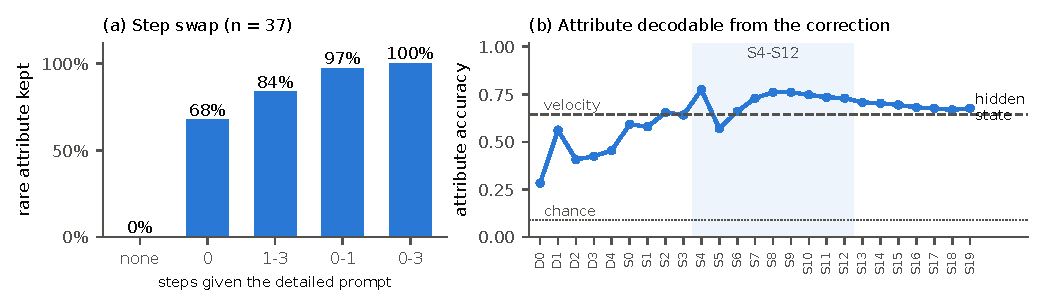
\includegraphics[width=\linewidth]{figs/decision.pdf}
\vspace{-1.6em}
\caption{\textbf{Where the attribute is decided.} (a)~Conditioning on the detailed prompt only at the listed steps of the
vanilla trajectory, 37 dev drift cases: steps 0--1 restore the attribute in 97\% of cases. (b)~Leave-one-subject-out accuracy of
decoding the rare attribute (11 classes) from the subject-pooled correction $\dH_l$ at step 0, per block. It peaks at S4 (0.77),
above velocity space (0.65).}
\label{fig:decision}
\end{figure*}

\section{Where the attribute is lost}
For a drifted case we evaluate both prompts at the same $x_t$ along the vanilla trajectory and take the difference
$\dv=v(x_t,c_\text{detailed})-v(x_t,c_\text{vanilla})$, and $\dH_l$ for the hidden states of block $l$.

\paragraph{Timing.} Swapping in the detailed prompt at steps 0--1 only restores the attribute in 97\% of cases, at step~0
only in 68\% (Fig.~\ref{fig:decision}a). The correction is large early and fades: $\|\dv\|/\|v\|$ is 0.41, 0.33, 0.19 and 0.10
over the four steps, and the top 10\% of tokens, on the subject, carry 49\% of $\|\dv_0\|^2$.

\paragraph{Direction.} The correction is not one universal direction. Subject-pooled $\dv_0$ of unrelated cases are orthogonal
(mean cosine 0.03), while cases sharing the rare attribute agree (0.55). The attribute is most linearly decodable from
$\dH_l$ in the middle single-stream blocks, S4--S12 (Fig.~\ref{fig:decision}b).

\paragraph{The model sees the attribute.} Without any label, a ridge classifier on the model's own pooled activations of the
reference image's subject (block S8, step 0) names the rare attribute of unseen subjects with 69\% top-1 and 92\% top-3
accuracy over 11 attributes (majority class 21\%; 226 cases). Colour (88\%) and gender (100\%) are read well, pattern (26\%)
and place (0\%) are not. The model therefore reads the purple banana as purple and still renders it yellow.

\section{Fixing drift without rewriting the prompt}
\paragraph{Methods.} \emph{Hidden-state steering} adds, at blocks S4--S12 and steps 0--1, the mean $\dH_l$ of the same rare
attribute learned on other subjects, scaled by $\alpha=4$, to the top 25\% of generated-image tokens by attention to the
subject word (a mask read from the model, no segmentation). \emph{Velocity steering} adds the analogous mean $\dv$. These need
the attribute name, like the prompts, but leave the prompt unchanged. Label-free: a \emph{velocity-matching LoRA} (rank 16 on
S4--S12, active at steps 0--1) trained on dev to make $v(c_\text{vanilla})$ match the frozen model's $v(c_\text{detailed})$;
SDEdit~\citep{sdedit}, which starts from the noised reference; a boost of attention from the subject's image tokens to the
reference; and negative guidance away from the typical attribute. Text-difference guidance adds
$2\,(v(c_\text{attr})-v(c_\text{vanilla}))$ at steps 0--1 and is a prompt-side baseline.

\begin{table*}[t]
\centering\small
\begin{tabular}{@{}lccccclc@{}}
\toprule
Method & Label & Passes & Kept & Edited & Defect & Clean [95\% CI] & Judge 2 \\
\midrule
Detailed prompt & prompt & 0 & 95 & 97 & 0 & \textbf{92} [86, 96] & 67 \\
Minimal attribute prompt & prompt & 0 & 93 & 94 & 0 & \textbf{87} [80, 93] & 65 \\
Text-difference guidance & yes & 2 & 93 & 94 & 0 & \textbf{87} [81, 92] & 58 \\
Hidden-state steering (S4--S12) & yes & 1 & 79 & 97 & 8 & \textbf{71} [64, 77] & 48 \\
Velocity steering & yes & 1 & 64 & 94 & 3 & \textbf{57} [47, 65] & 41 \\
\midrule
Velocity-matching LoRA & no & 0 & 51 & 96 & 1 & \textbf{47} [37, 57] & 34 \\
SDEdit, skip 1 step & no & $-1$ & 42 & 85 & 2 & \textbf{34} [26, 43] & 16 \\
Negative guidance & typical & 2 & 21 & 99 & 1 & \textbf{20} [15, 26] & -- \\
Reference-attention boost & no & 1 & 7 & 97 & 0 & \textbf{6} [3, 10] & -- \\
Vanilla prompt & no & 0 & 0 & 99 & 0 & \textbf{0} [0, 0] & 1 \\
\bottomrule
\end{tabular}
\caption{\textbf{Held-out test}: 233 drifting rare-view cases from 70 subjects not used for any choice. Label: whether the
method needs the rare attribute (``typical'': needs the typical one). Passes: extra transformer passes at the steered steps.
Kept, Edited, Defect: \% of cases by judge 1. Clean: all three; Judge 2: clean under the second judge, rescoring the same
images (``--'': not rescored).}
\label{tab:test}
\end{table*}

\paragraph{Results.} Table~\ref{tab:test} shows the held-out test results. Prompt-side methods reach 87--92\%; hidden-state steering reaches 71\%
[64,~77], the best method that leaves the prompt unchanged; the best label-free method, the LoRA, reaches 47\%. The second judge
is stricter on every method but preserves the order, and steering stays 17 points [10,~25] below the minimal prompt. By type
(Table~\ref{tab:types}), steering nearly matches prompts on pattern and is close on colour, but fails on gender and age, which
are not local appearance changes. The LoRA fixes colour and pattern on seen attributes but only 38\% of drifts on
attributes absent from training, against 79\% for the minimal prompt.

\begin{table}[t]
\centering\small
\setlength{\tabcolsep}{4pt}
\resizebox{\linewidth}{!}{\begin{tabular}{@{}lrccccc@{}}
\toprule
Type & $n$ & Min.\ prompt & Hidden steer. & Vel.\ steer. & LoRA & SDEdit \\
\midrule
Colour & 118 & 92 & 78 & 76 & 50 & 26 \\
Pattern & 56 & 91 & 88 & 54 & 73 & 57 \\
Material & 22 & 45 & 41 & 23 & 9 & 18 \\
Gender & 18 & 94 & 33 & 11 & 17 & 33 \\
Age & 11 & 82 & 36 & 0 & 18 & 18 \\
State & 8 & 100 & 75 & 62 & 25 & 62 \\
\bottomrule
\end{tabular}}
\caption{Test clean success (\%) by attribute type, judge 1.}
\label{tab:types}
\end{table}

\section{Why image-side fixes are capped}
Steering could fall short because its directions are poor or because of where it acts. We separate the two with oracles on dev
(Fig.~\ref{fig:ceiling}). For each case we run the detailed prompt at the same $x_t$ and pull the vanilla run's generated-image
tokens towards it at S4--S12, steps 0--1: exactly (every token), through the top-$k$ singular directions of the per-token
difference, or as the case's \emph{own} pooled correction, the best any steering vector could do.

\begin{figure}[t]
\centering
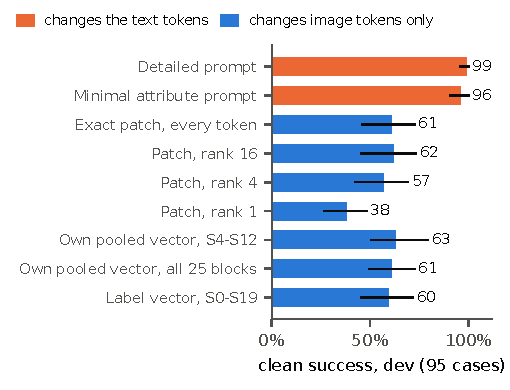
\includegraphics[width=\linewidth]{figs/ceiling.pdf}
\vspace{-1.8em}
\caption{\textbf{Oracle ceiling} on the 95 dev cases fixed by the detailed prompt. Patch: the generated-image tokens at S4--S12,
steps 0--1, are replaced by (a low-rank part of) their detailed-prompt values. Own pooled vector: the case's own
subject-pooled correction ($\alpha=2$). Label vector: per-attribute direction from other subjects, S0--S19, $\alpha=4$.
Lines: 95\% CI.}
\label{fig:ceiling}
\end{figure}

\paragraph{Exact patching is not enough.} Making the generated-image tokens identical to the corrected run at S4--S12
recovers 61\% of these cases, against 99\% for the detailed prompt itself (50\% vs.\ 83\% on all 121 dev cases). Steps 2--3
are not the cause: the step swap shows that the detailed prompt at steps 0--1 alone suffices. The difference lies in what
the patch leaves untouched: the text tokens, which the remaining blocks S13--S19 keep attending to and which, under the
vanilla prompt, still encode the typical attribute.

\paragraph{Directions are not the bottleneck.} The case's own pooled correction (63\%) matches exact patching, and a rank-16
patch (62\%) already saturates it. Spreading the vector over all 25 blocks (61\%) does not raise the ceiling, and the label direction learned on other subjects
(S0--S19, 60\%) is already within 3 points of it. Better directions therefore cannot close the gap to prompting; it comes from
the text stream.

\paragraph{Label-free attempts.} Table~\ref{tab:labelfree} lists every label-free family we tried on the same 121 dev cases.
Injecting the reference into the subject's $\hat x_0$ at step 1 on top of SDEdit is the best (52--57\%), but it trades edits
for attributes and drops to 26--31\% under the second judge. Approaches that amplify what the model already does with the
reference fail outright: reference guidance $v + w\,(v(\text{ref})-v(\text{no ref}))$ reaches 21\%, and boosting attention from
the subject word's \emph{text} tokens to the reference subject reaches 15\%, although both visibly change the output (mean
pixel change 10--33/255).
Predicting the correction from the reference activations matches the true correction better than the label direction
(cosine 0.59 vs.\ 0.47) yet steers worse (31\%), and SHIFT-style text-token steering~\citep{shift} with directions from
contrastive prompts reaches 31\%. In the first two steps the rare attribute is not present in the velocity in a form these
methods can amplify; restating it in the prompt is what puts it there.

\begin{table}[t]
\centering\small
\setlength{\tabcolsep}{3.5pt}
\resizebox{\linewidth}{!}{\begin{tabular}{@{}llrl@{}}
\toprule
Method & Label & $n$ & Clean [95\% CI] \\
\midrule
Minimal attribute prompt & label & 121 & \textbf{87} [78, 94] \\
Detailed prompt & label & 121 & \textbf{83} [70, 91] \\
Hidden-state steering, S4--S12 & label & 109 & \textbf{49} [30, 63] \\
\midrule
Source injection + edit guidance & no & 121 & \textbf{57} [43, 70] \\
Source injection & no & 121 & \textbf{52} [40, 63] \\
SDEdit, skip 1 step & no & 121 & \textbf{34} [21, 48] \\
Correction predicted from reference & no & 121 & \textbf{31} [21, 40] \\
Text-token steering (SHIFT-style) & contrast pairs & 121 & \textbf{31} [18, 47] \\
Reference guidance & no & 121 & \textbf{21} [11, 33] \\
Probe names attribute, then steering & no & 121 & \textbf{20} [13, 32] \\
Text-to-reference attention boost & no & 121 & \textbf{15} [8, 21] \\
Vanilla prompt & no & 121 & \textbf{3} [0, 7] \\
\bottomrule
\end{tabular}}
\caption{\textbf{Dev}, 121 type-balanced drift cases, judge 1. For each label-free family, the best of its settings on
these same cases is shown, so these numbers are optimistic. $n$: cases where the method applies.}
\label{tab:labelfree}
\end{table}

\begin{figure*}[t]
\centering
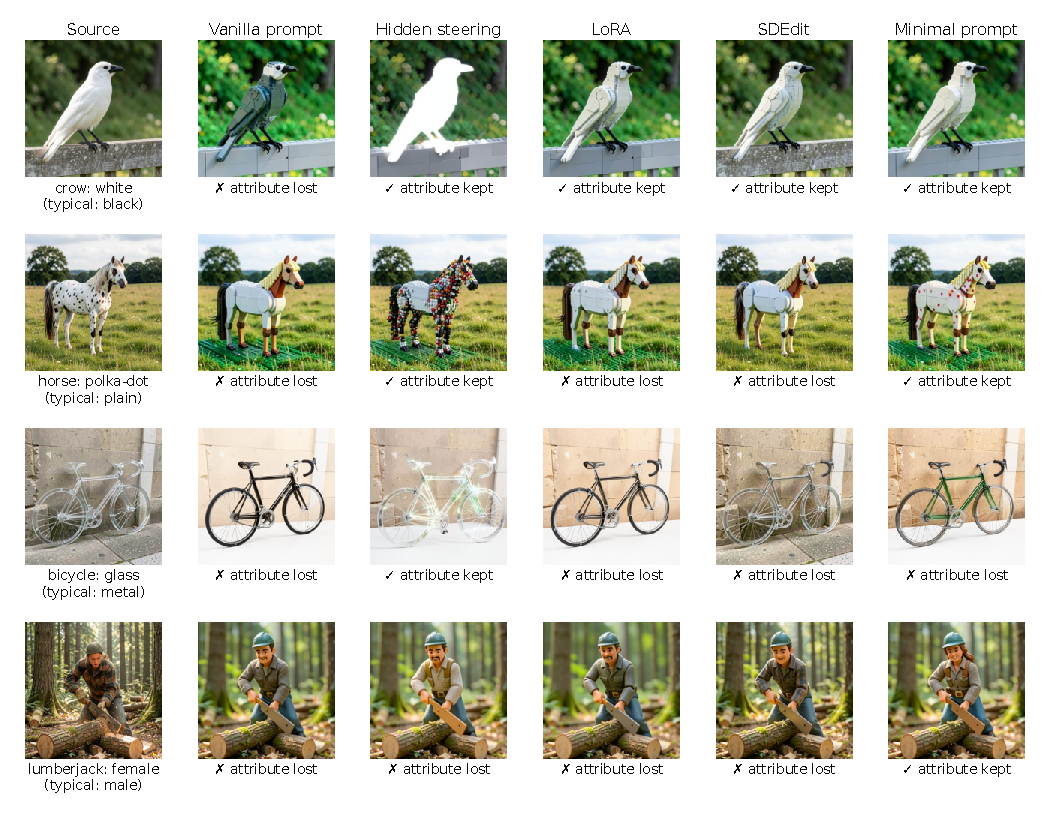
\includegraphics[width=0.92\linewidth]{figs/examples.pdf}
\vspace{-0.6em}
\caption{\textbf{Test examples}: the first case (by id) of four attribute types, not selected on outcome. Labels are judge 1.
Judge 1 accepts the hidden-steering crow, whose features are erased; judge 2 flags it as a defect, an example of the evaluation
noise discussed in Sec.~\ref{sec:limits}.}
\label{fig:examples}
\end{figure*}

\section{Related work}
SHIFT~\citep{shift} steers text-token activations of FLUX.1 with mean-difference and SVM directions to erase, add or switch concepts
in text-to-image generation; our steering belongs to the same family but targets image tokens in reference editing, and our
oracle results bound what such vectors can achieve there. Activation addition~\citep{actadd} introduced inference-time steering in
language models. R2F~\citep{r2f} addresses rare concepts in text-to-image by alternating rare and frequent prompts in early steps,
consistent with our finding that the first steps decide. Attend-and-Excite~\citep{attendexcite} and Prompt-to-Prompt~\citep{p2p}
manipulate cross-attention to control which concepts appear; our attention boosts are of this kind and do not fix drift.
SDEdit~\citep{sdedit} and Stable Flow~\citep{stableflow} preserve the source by trajectory or layer injection; we find that this
keeps attributes only at the cost of the edit. FLUX.1 Kontext~\citep{kontext} reports drift over repeated edits; we study a
single edit and a specific cause, the attribute prior.

\section{Limitations}\label{sec:limits}
All scores come from VLM judges. ``Edit applied'' is the weakest measurement ($\kappa=0.46$ between judges), and judge 1 misses
some defects (Fig.~\ref{fig:examples}); human labels are needed for absolute numbers. We study one step-distilled model with four
steps. The test split was used for two evaluation rounds (steering with baselines, then the LoRA) and for rescoring with judge 2.
The analysis and label-free experiments are on dev only, and Table~\ref{tab:labelfree} shows the best setting of each family.
Rare-view pairs were selected because they drifted at the dataset seed, which inflates drift rates at that seed.

\section{Conclusion}
Attribute drift in FLUX.2 [klein] edits happens in the first two steps, while the model still encodes the rare attribute of the
reference. Image-token steering recovers most colour and pattern drifts but is capped near what exact patching achieves,
because the text tokens keep re-imposing the typical attribute in later blocks. A fix without the label has to change what the
text stream says about the subject, for instance by writing what the model reads from the reference into the subject's text
tokens, rather than amplifying the reference on the image side.

\paragraph{Code.} Code, per-case results and figure scripts are available at\\
\url{https://github.com/Diaa340/rare-attribute-drift}.

{\small
\bibliographystyle{abbrvnat}
\bibliography{refs}
}

\appendix
\section{Two judges on the label-free dev methods}
\begin{table}[h]
\centering\small
\setlength{\tabcolsep}{3pt}
\resizebox{\linewidth}{!}{\begin{tabular}{@{}lcccccc@{}}
\toprule
 & \multicolumn{3}{c}{Judge 1} & \multicolumn{3}{c}{Judge 2} \\
\cmidrule(lr){2-4}\cmidrule(l){5-7}
Method & Kept & Edited & Clean & Kept & Edited & Clean \\
\midrule
Minimal attribute prompt & 92 & 98 & \textbf{87} & 84 & 77 & \textbf{65} \\
Detailed prompt & 85 & 98 & \textbf{83} & 83 & 82 & \textbf{65} \\
Source injection + edit guidance & 75 & 82 & \textbf{57} & 66 & 52 & \textbf{31} \\
Source injection & 78 & 76 & \textbf{52} & 71 & 46 & \textbf{26} \\
SDEdit, skip 1 step & 62 & 72 & \textbf{34} & 60 & 49 & \textbf{24} \\
Vanilla prompt & 3 & 98 & \textbf{3} & 5 & 84 & \textbf{4} \\
\bottomrule
\end{tabular}}
\caption{121 dev drift cases scored by both judges (\%).}
\end{table}

\end{document}
